\documentclass[9pt]{beamer}

\usepackage[T1]{fontenc}
\usepackage[utf8]{inputenc}
\usepackage[frenchb]{babel}
\usepackage{eurosym}

\usepackage{multirow}

\usepackage{graphicx}


\newcommand\host{{\it host} }
\newcommand\device{{\it device} }

\newcommand{\stream}{{\tt stream} }


% --------- BEGIN STYLE BEAMER ---------
\usetheme{Madrid}
\definecolor{ECNBleu}{HTML}{102648}
\definecolor{ECNJaune}{HTML}{FAB600}

\setbeamercolor{frametitle}{bg=ECNBleu,fg=white} %le titre de la frame, en haut
\setbeamercolor{title in head/foot}{bg=ECNJaune,fg=ECNBleu} %barre bas, milieu
\setbeamercolor{author in head/foot}{bg=ECNBleu,fg=ECNJaune} %barre bas, gauche
\setbeamercolor{date in head/foot}{bg=ECNBleu,fg=ECNJaune} %barre bas, droit
\setbeamercolor{section in head/foot}{bg=ECNJaune,fg=ECNBleu} %haut gauche
\setbeamercolor{subsection in head/foot}{bg=ECNBleu,fg=ECNBleu} %haut droite
\setbeamercolor{title}{bg=ECNBleu,fg=white}
\setbeamercolor{block title}{fg=white,bg=ECNBleu}

%\setbeamercolor{normal text}{bg=IUTBleuFonce} %texte
\setbeamercolor{item}{bg=ECNBleu}
\setbeamercolor{subitem}{bg=ECNJaune}
\setbeamercolor{description item}{fg=couleurEmph}
\setbeamercolor{section in toc}{fg=ECNBleu}
%\setbeamercolor{subsubitem}{bg=IUTBleuFonce}

%structure (eq emph dans beamer)
\setbeamercolor{emph}{fg=couleurEmph}
% ----------------------------

\usepackage{listings}

\lstdefinestyle{customc}{
  belowcaptionskip=1\baselineskip,
  breaklines=true,
  frame=L,
  xleftmargin=\parindent,
  language=C,
  showstringspaces=false,
  basicstyle=\tiny\ttfamily,
  keywordstyle=\bfseries\color{green!40!black},
  commentstyle=\itshape\color{purple!40!black},
  identifierstyle=\color{blue},
  stringstyle=\color{orange},
}

\lstset{escapechar=@,style=customc}

\newenvironment<>{questionblock}[1]{%
\setbeamercolor{block title}{bg=ECNJaune,fg=ECNBleu}%
\begin{block}#2{#1}}{\end{block}}

\title[GPGPU]{Programmation sur Processeur Graphique}

\subtitle[\ldots]{
---\\Partie 11 : Streams}
\author[P.-E. Hladik]{Pierre-Emmanuel Hladik\\\tiny pierre-emmanuel.hladik@ec-nantes.fr}
\institute[Centrale Nantes]{}
\date{\today}

\begin{document}

\frame{\titlepage}

%%%%%%%%%%%%%%%%%%%%%%%%%%
\begin{frame}[plain]
\frametitle{Transfert de données et calcul sérialisés}

      \centering
      \begin{block}{Exemple {\tt VecAddKernel()}}
		{\tt cudaMemcpy} sérialise le transfert de données et le calcul GPU 
	\end{block}  
	
	\begin{center}
		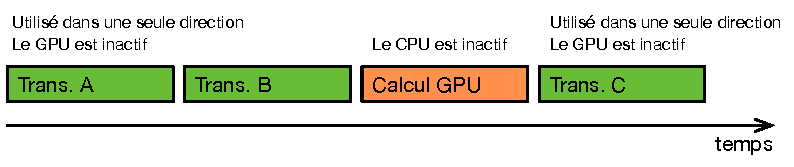
\includegraphics[width=.8\textwidth]{./figures-pdf/serialisation}
	\end{center}
\end{frame}
%%%%%%%%%%%%%%%%%%%%%%%%%%
\begin{frame}[plain, fragile]
\frametitle{{\tt Device Overlap}}

      \begin{block}{Exemple {\tt VecAddKernel()}}
		Certains périphériques CUDA permettent l'exécution simultanée d'un kernel tout en copiant des données entre le périphérique et la mémoire hôte.
	\end{block}  

\begin{lstlisting}[language=C]
int dev_count;
cudaDeviceProp prop;
cudaGetDeviceCount( &dev_count);

for (int i = 0; i < dev_count; i++) {
	cudaGetDeviceProperties(&prop, i);
	if (prop.deviceOverlap)
	...
 \end{lstlisting}
\end{frame}
%%%%%%%%%%%%%%%%%%%%%%%%%%
\begin{frame}[plain]
\frametitle{Fonctionnement idéale en pipeline}


      \centering
      \begin{block}{Exemple {\tt VecAddKernel()}}
		\begin{itemize}
			\item Diviser les grands vecteurs en segments
			\item Superposer les transferts et les calculs des segments adjacents
		\end{itemize}
	\end{block}  
	
	\begin{center}
		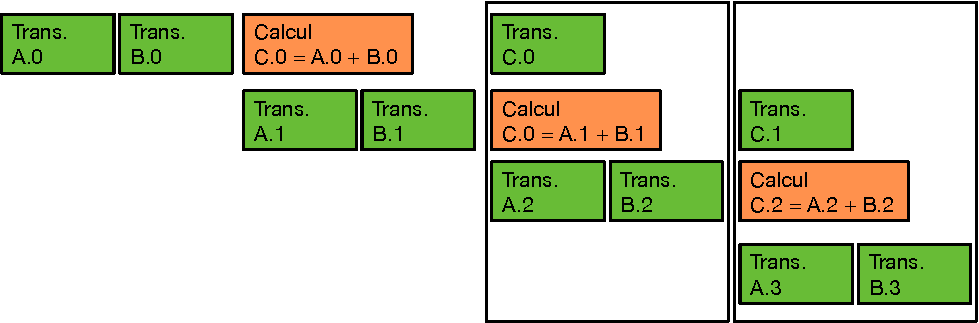
\includegraphics[width=.8\textwidth]{./figures-pdf/pipeline}
	\end{center}
\end{frame}
%%%%%%%%%%%%%%%%%%%%%%%%%%
\begin{frame}[plain]
\frametitle{Concurrence par le biais du pipeling}

	\begin{center}
		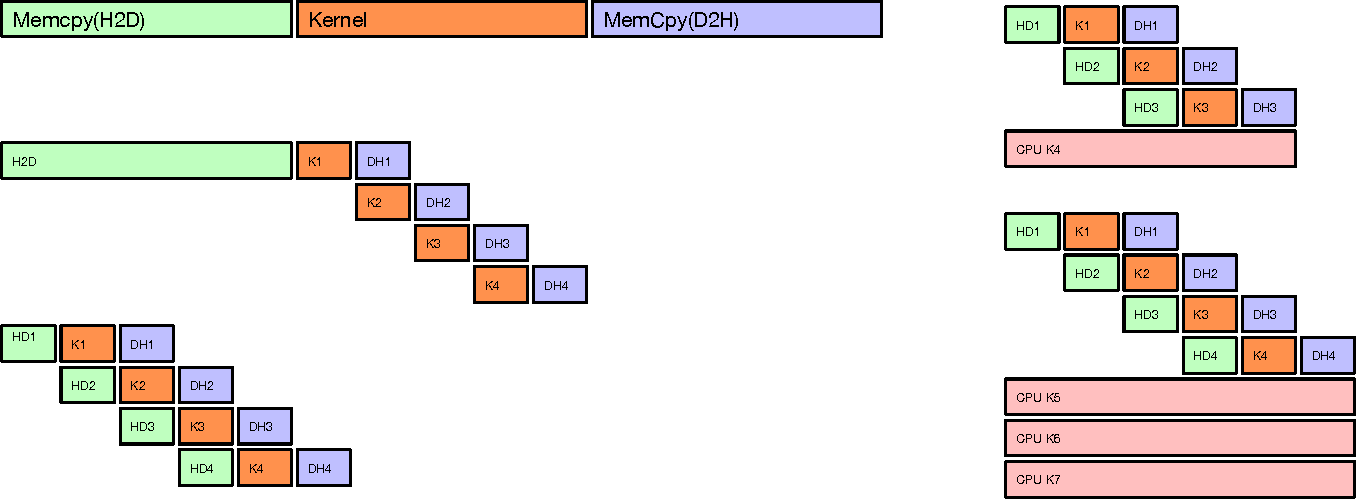
\includegraphics[width=.95\textwidth]{./figures-pdf/pipeline2}
	\end{center}
\end{frame}
%%%%%%%%%%%%%%%%%%%%%%%%%%
\begin{frame}[plain]
\frametitle{Synchronicité en CUDA}

      \begin{block}{Synchrone vs asynchrone}
	Tous les appels CUDA sont soit synchrones, soit asynchrones par rapport à l'hôte :
		\begin{itemize}
			\item Synchrone : mise en file d'attente du travail et attente de sa terminaison
			\item Asynchrone : mise en file d'attente du travail et retour immédiat\medskip
		\end{itemize}
	\end{block}  

      \begin{alertblock}{}
	Le lancement d'un kernel est asynchrone et se recouvre ({\it overlap}) automatiquement avec l'hôte
	\end{alertblock}  

\end{frame}
%%%%%%%%%%%%%%%%%%%%%%%%%%
\begin{frame}[plain]
\frametitle{Les streams CUDA }

CUDA prend en charge l'exécution parallèle des kernels et de {cudaMemcpy} avec des {\it \bf streams} :
\medskip
	\begin{itemize}
		\item Chaque {\it stream} est une file d'attente d'opérations sur le device (lancements de kernels et appels à {\tt cudaMemcpy}) :
			\begin{itemize}
				\item L'hôte place le travail dans la file d'attente et continue immédiatement
				\item Le device planifie le travail à partir des streams lorsque les ressources sont libres
			\end{itemize}
			\medskip
		\item Les opérations (tâches) de différents {\tt streams} peuvent être exécutées en parallèle (parallélisme des tâches) :
				 Mem CPU->GPU // Mem CPU-> GPU // kernel
			
	\end{itemize}

\end{frame}
%%%%%%%%%%%%%%%%%%%%%%%%%%
\begin{frame}[plain]
\frametitle{Ordre execution d'un stream}

Les demandes faites par l'hôte sont placées dans des files d'attente de type \og premier entré, premier sorti \fg\,(FIFO) :
\medskip
	\begin{itemize}
		\item Les files d'attente sont lues et traitées de manière asynchrone par le pilote et le device.
		\medskip
		\item Le pilote s'assure que les opérations dans une file d'attente sont traitées en séquence. Par exemple, les copies de mémoire se terminent avant le lancement du noyau, etc.
	\end{itemize}

	\begin{center}
		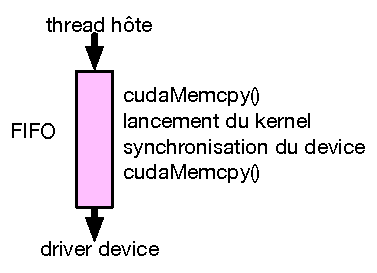
\includegraphics[scale=.8]{./figures-pdf/FIFO_stream}
	\end{center}

\end{frame}
%%%%%%%%%%%%%%%%%%%%%%%%%%
\begin{frame}[plain]
\frametitle{Execution de plusieurs streams}

	\begin{itemize}
		\item Pour permettre le parallèlisme des transferts mémoire et de l'exécution des noyau, il faut utiliser plusieurs {\it streams}
	\end{itemize}

	\begin{center}
		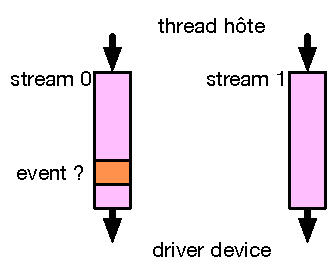
\includegraphics[scale=.8]{./figures-pdf/multi_streams}
	\end{center}
	
	\begin{itemize}
		\item Les événements CUDA permettent au thread hôte d'interroger et de se synchroniser avec des files d'attente individuelles (c'est-à-dire des {\it streams})
	\end{itemize}

\end{frame}
%%%%%%%%%%%%%%%%%%%%%%%%%%
\begin{frame}[plain]
\frametitle{Vue conceptuelle de l'exécution des streams}

	\begin{center}
		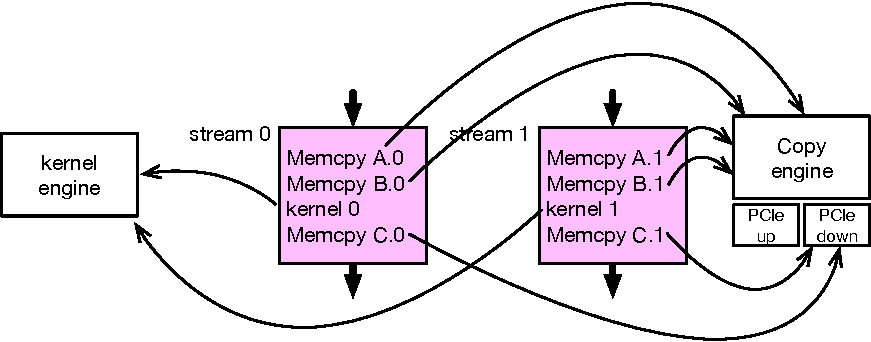
\includegraphics[scale=.8]{./figures-pdf/execution_calls}
	\end{center}

	\begin{itemize}
		\item Les traitements sont dépliés dans chaque FIFO (kernel, copy up, copy down)
		\item ... {\bf et l'ordre d'exécution est maintenu dans chaque stream}
	\end{itemize}


\end{frame}
%%%%%%%%%%%%%%%%%%%%%%%%%%
\begin{frame}[plain, fragile]
\frametitle{Gérer les {\it streams}}

\begin{itemize}
	\item Déclaration d'un gestionnaire de {\it stream} :
	\begin{lstlisting}[language=C]
cudaStream_t stream;
	 \end{lstlisting}
 
 	\item Allocation d'un {\it stream} :
	 \begin{lstlisting}[language=C]
 cudaStreamCreate(&stream);
	 \end{lstlisting}
 
 	\item Désallocation d'un {\it stream}
	\begin{lstlisting}[language=C]
cudaStreamDestroy(stream);
	\end{lstlisting} 
	Synchronise l'hôte jusqu'à ce que le travail du {\it stream} soit terminé
	
\end{itemize}
\end{frame}
%%%%%%%%%%%%%%%%%%%%%%%%%%
\begin{frame}[plain, fragile]
\frametitle{Placer un travail dans un {\it stream}}

\begin{itemize}
	\item Placer un kernel (4e paramètre) :
	\begin{lstlisting}[language=C]
		kernel<<< blocks , threads, smem, stream>>>();
	 \end{lstlisting}
 
	 \item Placer une copie de données :
	 \begin{lstlisting}[language=C]
		cudaMemcpyAsync( dst, src, size, dir, stream);
	 \end{lstlisting}

\end{itemize}
\end{frame}
%%%%%%%%%%%%%%%%%%%%%%%%%%
\begin{frame}[plain, fragile]
\frametitle{{\it stream} par défaut}

\begin{itemize}
	\item Sauf indication contraire, tous les appels sont placés dans un {\it stream} par défaut, souvent appelé \og {\it stream 0} \fg\medskip
	\item Le {\it stream 0} a des règles de synchronisation spéciales :
	\begin{itemize}
		\item Synchrone avec tous les streams : les opérations dans le {\it stream 0} ne peuvent pas chevaucher les autres streams\medskip
	\end{itemize}
	
	\begin{lstlisting}[language=C]
cudaStream_t stream1;
cudaStreamCreate(&stream1);

foo<<<blocks,threads>>>(); // Stream par defaut
foo<<<blocks,threads,0,stream1>>>(); // pas de concurrence dans ce cas

cudaStreamDestroy(stream1);
	 \end{lstlisting}

\end{itemize}

%\begin{itemize}
%	\item Exception : {\it stream} avec drapeau non-bloquant à l'allocation
%\begin{lstlisting}[language=C]
%cudaStreamCreateWithFlags(&stream,cudaStreamNonBlocking) 
%	 \end{lstlisting}
%	\begin{itemize}
%		\item Utilisé pour obtenir la concurrence avec des bibliothèques hors de votre contrôle
%	\end{itemize}
%		\begin{lstlisting}[language=C]
% cudaStream_t stream2;
%cudaStreamCreateWithFlags(&stream2,cudaStreamNonBlocking);
%
%foo<<<blocks,threads>>>(); // Stream par defaut
%foo<<<blocks,threads,0,stream2>>>();  // Concurrence d'execution
%
%cudaStreamDestroy(stream2);
%	 \end{lstlisting}
%\end{itemize}
\end{frame}
%%%%%%%%%%%%%%%%%%%%%%%%%%
\begin{frame}[plain, fragile]
\frametitle{Exemple de code pour gérer les streams}


	\begin{lstlisting}[language=C]
	// Declaration
	cudaStream_t stream1, stream2;
	
	// Instanciation
	cudaStreamCreate(&stream1);
	cudaStreamCreate(&stream2);

	// Affectation des kernels aux streams
	foo<<<blocks,threads,0,stream1>>>();
	foo<<<blocks,threads,0,stream2>>>();

	// Destrcution des streams
	cudaStreamDestroy(stream1);
	cudaStreamDestroy(stream2);
	 \end{lstlisting}

\end{frame}
%%%%%%%%%%%%%%%%%%%%%%%%%%
\begin{frame}[plain, fragile]
\frametitle{Copies concurrentes de la mémoire}

\begin{itemize}
	\item {\tt cudaMemcpy(...)}
	\begin{itemize}
		\item Le transfert mémoire est fait dans le {\tt stream 0} par défaut
		\item Est synchrone (i.e. doit être terminé avant son retour)\medskip
	\end{itemize}
	
	\item {\tt cudaMemcpyAsync(..., \&stream)}
	\begin{itemize}
		\item Place le transfert mémoire dans le stream et retourne immédiatement\medskip
	\end{itemize}

	\item La concurrence s'obtient si :
		\begin{itemize}
		\item les transferts se font dans un stream qui n'est pas celui par défaut
		\item les copies sont asynchrones
		\item un seul transfert par direction à la fois
		\item la mémoire de l'hôte est {\it pinned}
	\end{itemize}

\end{itemize}
\end{frame}
%%%%%%%%%%%%%%%%%%%%%%%%%%
\begin{frame}[plain, fragile]
\frametitle{Code hôte pour un simple Multi-Stream}

\begin{lstlisting}[language=C]
cudaStream_t stream1, stream2;

cudaStreamCreate(&stream1);
cudaStreamCreate(&stream2);

float *d_A1, *d_B1, *d_C1; // device memory for stream 1 
float *d_A2, *d_B2, *d_C2; // device memory for stream 2

// cudaMalloc() calls for d_A1, d_B1, d_C1, d_A2, d_B2, d_C2 go here
// h_A, h_B and h_C : vector on host

for (int i=0; i<n; i+=2*SegSize) { // n vector size, SegSize size of the segment (divisor of n)

	// Gestion stream 1
	cudaMemcpyAsync(d_A1, h_A+i, SegSize*sizeof(float), cudaMemcpyHostToDevice, stream1);
	cudaMemcpyAsync(d_B1, h_B+i, SegSize*sizeof(float), cudaMemcpyHostToDevice, stream1);
	vecAdd<<<SegSize/256, 256, 0, stream1>>>(d_A1, d_B1, d_C1);
	cudaMemcpyAsync(h_C+i, d_C1, SegSize*sizeof(float),cudaMemcpyDeviceToHost, stream1);

	// Gestion stream 2
	cudaMemcpyAsync(d_A2, h_A+i+SegSize, SegSize*sizeof(float), cudaMemcpyHostToDevice, stream2);
	cudaMemcpyAsync(d_B2, h_B+i+SegSize, SegSize*sizeof(float), cudaMemcpyHostToDevice, stream2);
	vecAdd<<<SegSize/256, 256, 0, stream2>>>(d_A2, d_B2, d_C2);
	cudaMemcpyAsync(h_C+i+SegSize, d_C2, SegSize*sizeof(float),cudaMemcpyDeviceToHost, stream2);
}

 \end{lstlisting}
\end{frame}
%%%%%%%%%%%%%%%%%%%%%%%%%%
\begin{frame}[plain]
\frametitle{Exécution des streams : mauvaise synchronisation}

	\begin{center}
		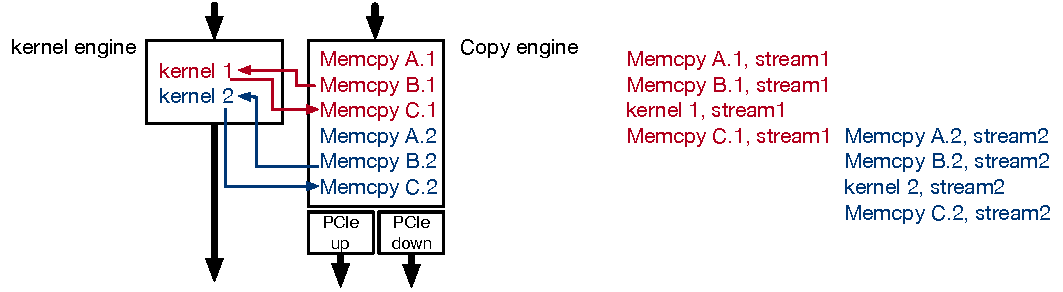
\includegraphics[width=\textwidth]{./figures-pdf/execution_calls2}
	\end{center}

	\begin{center}
		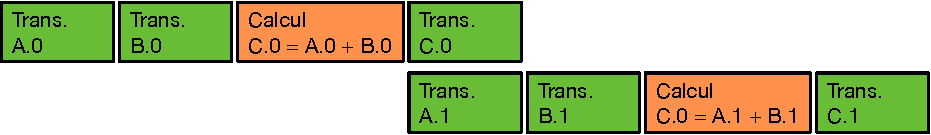
\includegraphics[scale=.7]{./figures-pdf/no_overlap}
	\end{center}

\end{frame}
%%%%%%%%%%%%%%%%%%%%%%%%%%
\begin{frame}[plain, fragile]
\frametitle{Code hôte avec une meilleure utilisation du Multi-Stream}

\begin{lstlisting}[language=C]
cudaStream_t stream1, stream2;

cudaStreamCreate(&stream1);
cudaStreamCreate(&stream2);

float *d_A1, *d_B1, *d_C1; // device memory for stream 1
float *d_A2, *d_B2, *d_C2; // device memory for stream 2

// cudaMalloc() calls for d_A1, d_B1, d_C1, d_A2, d_B2, d_C2 go here
// h_A, h_B and h_C : vector on host

for (int i=0; i<n; i+=2*SegSize) { // n vector size, SegSize size of the segment (divisor of n)

	// Entrelacement des copies memoire
	cudaMemcpyAsync(d_A1, h_A+i, SegSize*sizeof(float),cudaMemcpyHostToDevice, stream1);
	cudaMemcpyAsync(d_B1, h_B+i, SegSize*sizeof(float),cudaMemcpyHostToDevice, stream1);

	cudaMemcpyAsync(d_A2, h_A+i+SegSize, SegSize*sizeof(float),cudaMemcpyHostToDevice, stream2);
	cudaMemcpyAsync(d_B2, h_B+i+SegSize, SegSize*sizeof(float),cudaMemcpyHostToDevice, stream2);

	vecAdd<<<SegSize/256, 256, 0, stream1>>>(d_A1, d_B1, d_C1);		
	vecAdd<<<SegSize/256, 256, 0, stream2>>>(d_A2, d_B2, d_C2);

	cudaMemcpyAsync(h_C+i, d_C1, SegSize*sizeof(float),cudaMemcpyDeviceToHost, stream1);
	cudaMemcpyAsync(h_C+i+SegSize, d_C2, SegSize*sizeof(float),cudaMemcpyDeviceToHost, stream2);
}

 \end{lstlisting}
\end{frame}
%%%%%%%%%%%%%%%%%%%%%%%%%%
\begin{frame}[plain]
\frametitle{Exemple d'exécution des streams entrelacées}

	\begin{center}
		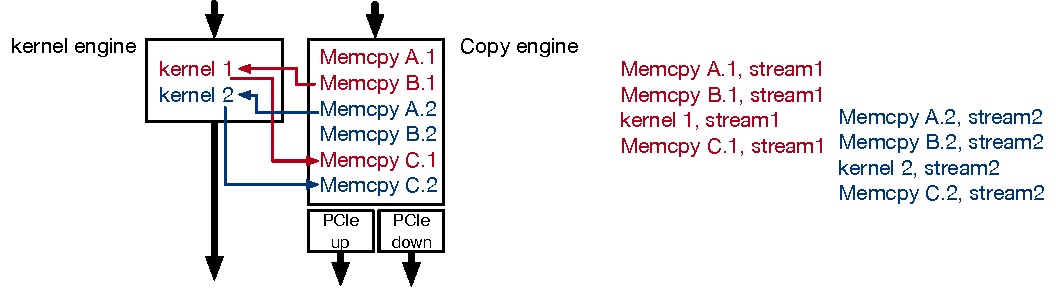
\includegraphics[width=\textwidth]{./figures-pdf/execution_calls3}
	\end{center}

	\begin{center}
		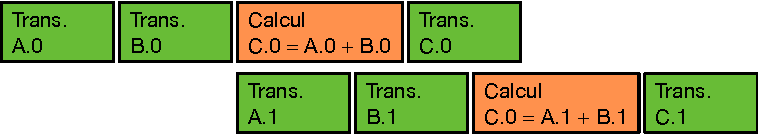
\includegraphics[scale=.7]{./figures-pdf/good_overlap}
	\end{center}

	\begin{center}
		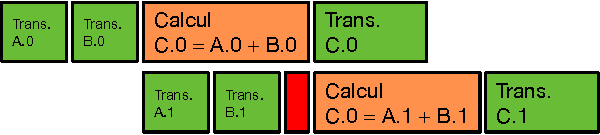
\includegraphics[scale=.7]{./figures-pdf/good_overlap2}
	\end{center}

\end{frame}
%%%%%%%%%%%%%%%%%%%%%%%%%%
\begin{frame}[plain, fragile]
\frametitle{Synchronisation}

	\begin{itemize}
		\item Tout synchroniser : bloque l'hôte jusqu'à ce que tous les appels CUDA émis soient terminés
		\begin{lstlisting}[language=C]
cudaDeviceSynchronize()
		 \end{lstlisting}
	 
		 \item Synchroniser l'hôte avec un flux spécifique : bloque l'hôte jusqu'à ce que tous les appels CUDA émis dans le stream soient terminés
		 \begin{lstlisting}[language=C]
cudaStreamSynchronize ( stream)
		 \end{lstlisting}
	 
		 \item Synchronisation de l'hôte ou des périphériques à l'aide d'événements
	\end{itemize}
\end{frame}

%%%%%%%%%%%%%%%%%%%%%%%%%%
%\begin{frame}[plain, fragile]
%\frametitle{gestion des {\it events}}
%
%	\begin{itemize}
%		\item {\tt cudaEventCreate(\&event)}
%		\begin{itemize}
%			\item Crée un évènement
%		\end{itemize}
%		\item {\tt cudaEventDestroy(\&event)} 
%		\begin{itemize}
%			\item Détruit un évènement
%		\end{itemize}
%
%		\item {\tt cudaEventCreateWithFlags(\&event, cudaEventDisableTiming)} 
%		\begin{itemize}
%			\item Désactive la synchronisation pour augmenter les performances et éviter des problèmes de synchronisation
%		\end{itemize}
%
%		\item {\tt cudaEventRecord(\&event, stream)}
%		\begin{itemize}
%			\item Définit l'état de l'événement comme non survenu
%			\item Met l'événement en file d'attente dans un stream
%			\item L'état de l'événement est défini comme étant survenu lorsqu'il atteint le début du stream
%		\end{itemize}
%
%	\end{itemize}
%\end{frame}
%%%%%%%%%%%%%%%%%%%%%%%%%%
%\begin{frame}[plain, fragile]
%\frametitle{Synchronisation en utilisant des événements}
%
%	\begin{itemize}
%		\item {\tt cudaEventQuery ( event )}
%		\begin{itemize}
%			\item Retourne CUDA\_SUCCESS si un événement s'est produit 
%		\end{itemize}
%		\item {\tt cudaEventSynchronize ( event )}
%		\begin{itemize}
%			\item Bloque l'hôte jusqu'à ce que le stream ait terminé tous les appels en cours 
%		\end{itemize}
%		\item {\tt cudaStreamWaitEvent ( stream, event )}
%		\begin{itemize}
%			\item Bloque le stream jusqu'à ce que l'événement se produise
%			\item Ne bloque les lancements qu'après cet appel 
%			\item Ne bloque pas l'hôte !
%		\end{itemize}
%	\end{itemize}
%	
%\begin{alertblock}{Erreur commune de multithreading}
%Appeler {\tt cudaEventSynchronize} avant {\tt cudaEventRecord}
%\end{alertblock}
%	
%\end{frame}

%%%%%%%%%%%%%%%%%%%%%%%%%%
\begin{frame}[plain, fragile]
\frametitle{Mémoire unifiée et stream}

Préfetching de données dans la mémoire unifiée CUDA :
	\begin{itemize}
		\item L'objectif principal est d'éviter les défauts de page
		\item Fournit un mécanisme pour améliorer les performances de l'application en établissant la localité des données
		\item Utilisé pour migrer les données vers un device ou l'hôte et mapper les tables de pages sur le processeur avant qu'il ne commence à utiliser les données.
%		\item Plus utile lorsque les données sont accessibles à partir d'un seul processeur
	\end{itemize}

\end{frame}
%%%%%%%%%%%%%%%%%%%%%%%%%%
\begin{frame}[plain, fragile]
\frametitle{API CUDA pour le prefetching de données}

{\tt \_\_host\_\_ cudaError\_t cudaMemPrefetchAsync ( const void* devPtr, size\_t count, int  dstDevice, cudaStream\_t stream = 0 )}
	\begin{itemize}
		\item {\tt devPtr} : Adresse de mémoire unifiée de la région de mémoire pour le prefectch
		\item {\tt count} : Taille en octets de la région du prefectch
		\item {\tt dstDevice} : Processeur de destination 
		\item {\tt stream} : stream CUDA\bigskip
	\end{itemize}
	

Remarques :
		\begin{itemize}
			\item Le prefetching est une opération asynchrone par rapport au device, mais l'appel peut ne pas être totalement asynchrone par rapport à l'hôte
			\item Le processeur de destination doit être un device ID ou cudaCpuDeviceId valide
			\item Si le processeur de prefetch est un GPU, la propriété du device cudaDevAttrConcurrentManagedAccess doit être différente de zéro
	\end{itemize}
\end{frame}
%%%%%%%%%%%%%%%%%%%%%%%%%%
\begin{frame}[plain, fragile]
\frametitle{Code hôte avec une meilleure utilisation du Multi-Stream}

\begin{lstlisting}[language=C]

// data must've been allocated with cudaMallocManaged( (void**) &data, N);

void function(int * data, cudaStream_t stream) {
	init(data, N);
	
	// Prefetch to the device cudaStreamSynchronize(stream);
	cudaMemPrefetchAsync(data, N * sizeof(int), myGpuId, stream);
	
	my_kernel<<<..., stream>>>(data, ...);
	
	// Prefetch to the host cudaStreamSynchronize(stream);
	cudaMemPrefetchAsync(data, N * sizeof(int), cudaCpuDeviceId, stream); 
	
	hostFunction(data, N);
}

 \end{lstlisting}
\end{frame}
%%%%%%%%%%%%%%%%%%%%%%%%%%

\begin{frame}[plain]
\frametitle{Un peu de pratique avec le TD 11}

\begin{block}{Objectifs}
\begin{itemize}
	\item Utilisation des streams
\end{itemize}
\end{block}
\end{frame}
%%%%%%%%%%%%%%%%%%%%%%%%%%

\end{document}